\documentclass{article}

\usepackage[utf8]{inputenc}
\usepackage[finnish]{babel}
\usepackage[T1]{fontenc}
\usepackage[kerning=true]{microtype}
\usepackage[citestyle=ieee]{biblatex}
\usepackage{lmodern}
\usepackage{amsmath}
\usepackage{amsfonts}
\usepackage{graphicx}
\newcommand{\code}{\texttt}

\bibliography{citations}

\title{Toteutusdokumentti}

\author{Sami Kukkonen}

\begin{document}

\section{Totetusdokumentti}

Järjestelmä muodostuu LZW-algoritmin \cite{Welch1} toteuttavista funktioista sekä tietorakenteista. Molemmat ovat toteutettu funktionaaliseen tyyliin sivuvaikutuksia ja mutaatioita välttäen. \cite[s. 39--60]{Chiusano1}
Pakkauslogiikka rakentuu \textbf{fs2}\footnote{\url{https://github.com/functional-streams-for-scala/fs2}} kirjaston päälle, kutsuen \code{Stream}-tyypille erinäisiä funktioita jotka muuttavat datavirtaa.
Pakkauslogiikka on jaettu kahteen tiedostoon: \code{Format.scala} pakkaa ja purkaa bittijonoja yksittäisten tavujen yli, ja tiedostossa \code{LZW.scala} olevat funktiot hoitavat itse sanakirjan ylläpitämisen ja koodien generoinnin.

Yhtenä projektin tavoitteena oli lisäksi saavuttaa yhteensopivus Unixin \code{compress}\footnote{\url{https://man.openbsd.org/compress.1}} -työkalun kanssa: \code{CompressHeader}-luokassa olevat funktiot lisäävät ja poistavat tiedoston alussa olevan tavujonon, jolla \code{compress} tunnistaa rakenteeltaan yhteensopivan tiedoston.

\subsection{Tietorakenteet}

LZW-algoritmin ydin tarvitsee toimiakseen jonkinlaisen hajautustaulutoteutuksen ja käytännössä
hajautustaulu sekä ohjelman monet osat käyttävät listaa aputietorakenteena. Molemmat on toteutettu
käyttäen \textit{trie}-nimistä tietorakennetta, joka on puurakenne, jonka lehdet vastaavat tietorakenteeseen
tallennettuja arvoja ja sisäsolmut vastaavat avainolion jotain osaa (esimerkiksi merkkijonossa tiettyä kirjainta tai yleisemmin
bittijonossa tiettyä osabittijonoa). \cite{Knuth1}

Tässä projektissa käytetty trie haarautuu puun joka tasolla
32 lapsisolmuun ja indeksoi tallennetut arvot pilkkomalla 32-bittisen kokonaisluvun bitit osabittijonoiksi, joiden avulla
reititys arvon sisältävään solmuun tapahtuu. Tällöin havaitaankin, että

\begin{itemize}
  \item rakenteeseen voi tallettaa enintään $2^{32}$ arvoa ja
  \item
    arvosolmun löytämisen aikavaativuus on $O(\log_{32} n)$. 32-bittisen kokonaisluvun suurin arvo on $2^{32}-1$, joten reititys
    tekee korkeintaan \\ $\log_{32}(2^{31}-1) \approx 6.4 = 7$ hyppyä.
\end{itemize}

\noindent Triellä siis toisin sanoen saavutetaan tilanne, jossa $O(\log n)$ aikavaativuudellinen tietorakenne kasvaa
aikavaativuudeltaan niin hitaasti, että useimmilla käytännön syötteillä rakenteen nopeus on lähestulkoon vakioaikainen. Trien toimintaa on havainnollistettu kuvassa \ref{fig:trie}.


Koska projektin tietorakenteet ovat toteutettu funktionaalisesti, ne eivät salli mutaatioita itseensä. Tällöin
arvon lisääminen listaan tai hajautustauluun vaatii uuden tietorakenteen luomista ilman että vanhaan rakenteeseen tulee muutoksia.
$n$-alkioisen taulukon käyttö vaatisi siis joka lisäyksen tai poiston yhteydessä kaikkien taulukon alkioiden kopioimista. Trie sen sijaan
mahdollistaa puun polkujen kierrättämisen tietorakenteiden välillä siten, että vain muuttunut polku juurisolmusta johonkin tiettyyn arvosolmuun
täytyy rakentaa uudelleen muutoksia tehdessä. Kun jokaisella puun tasolla on 32 lasta, on helppo nähdä, että jokainen päivitys
vaatii maksimissaan 6 32-bittisen taulukon rakentamista uudelleen. Tämä mahdollistaa tehokkaan muistinkäytön verrattuna koko rakenteen kopiointiin.


Projekti sisältää kaksi trietä käyttävää tietorakennetta: \code{HashMapVector}-luokan, joka pohjimmiltaan on vain kevyt
lisäys \code{SparseVector}in päälle kääntäen olion 32-bittiseksi kokonaisluvuksi jotain hajautusfunktiota käyttäen ja lisäten
ylivuotolistat mahdollisia hajautusarvotörmäyksiä varten.

Toinen trietä käyttävä tietorakenne on \code{ListVector}, joka tarjoaa listamaisen rajapinnan trien käyttöön.
Se siis varmistaa, että rakenteen avaimet eivät ole toisistaan erillään (rakenne on isomorfinen $i$-alkioisen linkitetyn listan kanssa),
mikä mahdollistaa listan ensimmäisen ja viimeisen alkion hakemisen $O(1)$ ajassa.
Toisaalta verrattuna normaaliin linkitettyyn listaan \code{ListVector} tarjoaa $O(\log n)$-nopeuksisen pääsyn mihin tahansa
alkioonsa.

Pakkausalgoritmi käyttää apuna myös \code{BitBuffer}-nimistä aputietorakennetta, joka on käytännössä listarajapinta
64-bittisen kokonaisluvun päälle. Sen avulla on mahdollista yhdistää useita bittijonoja yhdeksi bittijonoksi, mikä on kätevää
pakattaessa bittijonoja tavuiksi.

\begin{figure}
  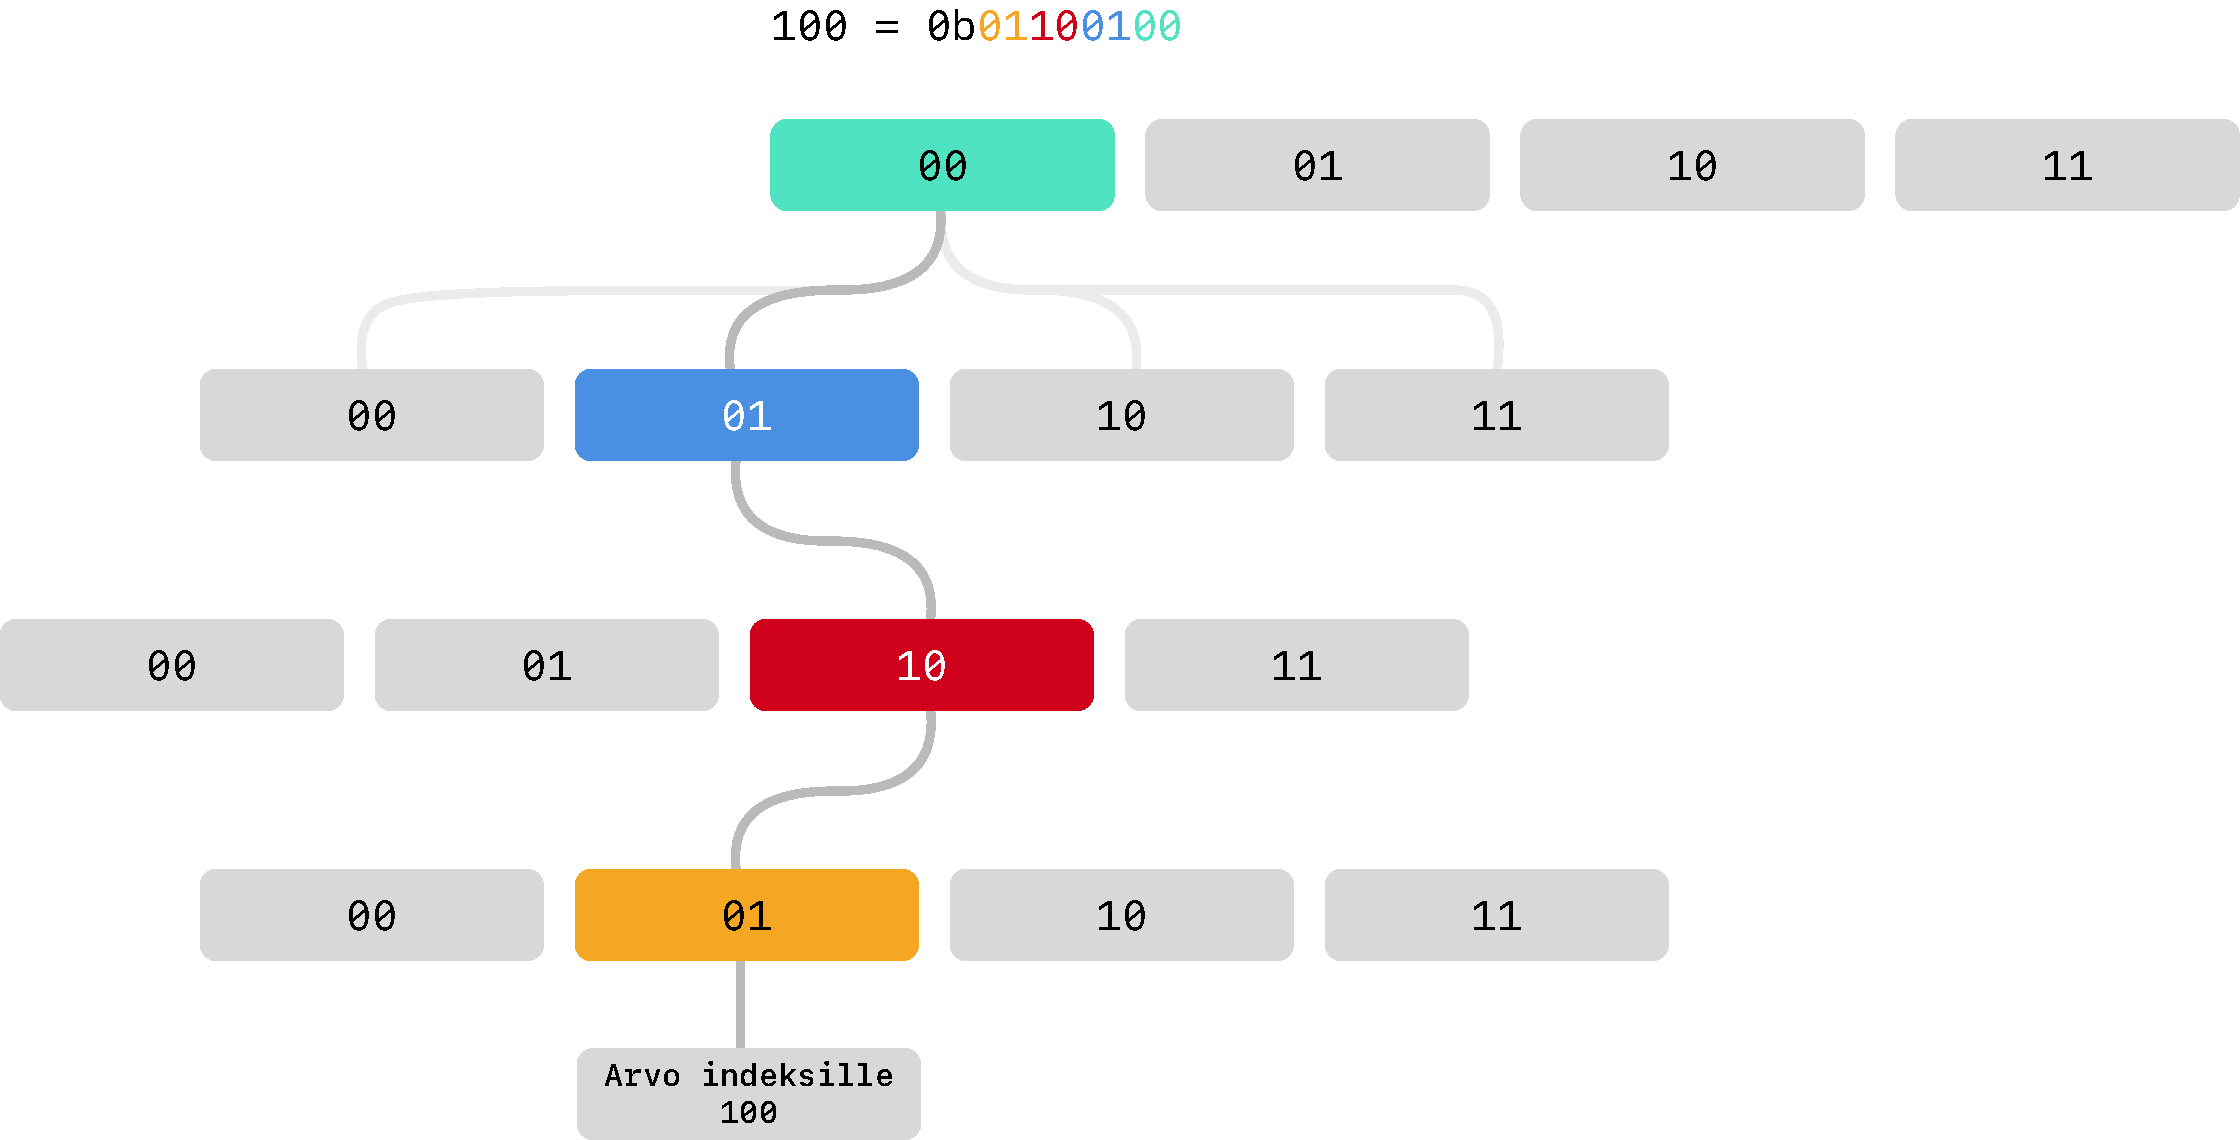
\includegraphics[width=\linewidth]{trie}
  \caption{Indeksin 100 arvon hakeminen bitti-indeksoidusta triestä, jonka haarautumisaste on 4. Koska 4 alkiolla voidaan esittää vain binääriluvut , luvun 100 binääriesitys pilkotaan 2 bitin pituisiin osajonoihin.}
  \label{fig:trie}
\end{figure}

\subsection{Funktionaalisesta ohjelmoinnista}

Yksi projektin päätavoitteesta oli harjaannuttaa funktionaalisessa ohjelmoinnissa. Sen vuoksi projektissa käytetään
huomattavasti \textbf{cats} \footnote{\url{https://github.com/typelevel/cats}}-kirjaston tarjoamia tyyppiluokkia (\textit{type class}), mitkä mahdollistavat
esimerkiksi algebrallisten rakenteiden mallinnuksen sekä toiminnallisuuden lisäämisen luokkiin loogisina kokonaisuuksina.
Näitä tyyppiluokkia voidaan ajatella rajapintoina, joita projektin eri komponentit toteuttavat.
Siten ne myös mahdollistavat selkeän erottelun järjestelmän eri osa-alueiden välille.

\subsection{Saavutetut aikavaativuudet}

Sekä hajautustaulurakenne että listarakenne saavuttavat ajassa $O(\log n)$ toimivan haun, lisäyksen sekä poiston trien avulla
(kts. luku 1.1). \code{BitBuffer}-rakenne käyttää bittioperaatiota toimintaansa, joten sen aikavaativuus em. operaatioille on O(1).
Järjestelmä pakkaa ja purkaa jonkin tiedoston yhdellä läpikäynnillä (\textit{single pass}), joten sen aikavaativuus on tällöin
$O(n \log n)$.

Käytännössä ohjelma on hyvin hidas verrattuna mihin tahansa moderniin pakkausalgoritmiin, joka on toteutettu imperatiivisesti. Empiirisen suorituskykytestauksen tulokset löytyvät testausdokumentista.

\printbibliography

\end{document}